
%(BEGIN_QUESTION)
% Copyright 2011, Tony R. Kuphaldt, released under the Creative Commons Attribution License (v 1.0)
% This means you may do almost anything with this work of mine, so long as you give me proper credit

When sulfur-containing fuels are burned, one of the reaction products is sulfur dioxide (SO$_{2}$), which is an atmospheric pollutant.  Fortunately, SO$_{2}$ is relatively easy to ``scrub'' out of hot flue gases by spraying a liquid solution down on the rising gases and then chemically treating (regenerating) that scrubbing solution:

$$\includegraphics[width=15.5cm]{i01992x01.eps}$$

The level control valve (LV) on this scrubber system has been recently rebuilt, but the technician who did the rebuild was not careful, and mis-calibrated the valve's bench-set.  Its bench-set pressure range is actually 4 to 16 PSI instead of 3 to 15 PSI like it's supposed to be.  Identify how this mis-calibration will affect the control of liquid level inside the scrubber, and also what you would need to do to the valve to correct the calibration error.  Be as specific as you can in your answers!

\underbar{file i01992}
%(END_QUESTION)





%(BEGIN_ANSWER)

No ill effect will result from this improper bench-set, except if the control valve needs to open fully and it cannot.  In that case, the liquid level might rise above setpoint.  {\it Award partial credit if the student does not also mention the possibility of liquid level rising under high-demand conditions, or if the student suggests the level will always be too high.}

\vskip 10pt

To correct this problem, you will need to {\it reduce} the compression of the valve spring slightly.  {\it Full credit should be given for identifying the spring adjustment, but no credit (for this half) should be given if the student thinks the valve stem coupling needs to be adjusted.}

%(END_ANSWER)





%(BEGIN_NOTES)

{\bf This question is intended for exams only and not worksheets!}.

%(END_NOTES)


